%   ------------------------------------------------------------------------
\FloatBarrier
\subsection{Funcionalidade de imagem para vídeo}
\label{s.vidu.imagem}

A funcionalidade de imagem para vídeo permite que o usuário defina o primeiro e, opcionalmente, o último frame do vídeo a ser gerado, além da clássica descrição do prompt, podendo especificar ações para diferentes quadros. 

Nos testes iniciais, o objetivo era criar uma animação das portas fechando ou abrindo (que ainda não havia sido feita na época). Nessa funcionalidade, não foi possível mais usar as referências criadas anteriormente, sendo possível apenas anexar uma imagem simples para os frames inicial e final. Utilizando as recomendações descobertas anteriormente, um prompt foi confeccionado para ser usado em todas as tentativas, que foi apenas levemente modificado de acordo com as necessidades.

Para a porta cinza, foi colocado o sprite dela aberta (Figura \ref{fig:viduPortaC3}) para o primeiro quadro, e a figura dela fechada (Figura \ref{fig:viduPortaC2}) para o último quadro. O resultado gerado\footnote{\url{https://drive.google.com/file/d/1MExWoA7CkPSTmd0MBEr3Z3-u9n4KmTfW/view?usp=sharing}} foi um sucesso parcial. A câmera se mexe de acordo com o movimento da porta, que foi distorcida a ponto de perder os detalhes das rachaduras e expandida na horizontal(Figura \ref{fig:viduPortaMaior}) antes de se fechar. Apesar disso, encontrou-se uma oportunidade de usar a animação como base para alguns ajustes, como adicionar as rachaduras novamente e manter a câmera fixa no mesmo ponto. Isso ocorreu pois o movimento de fechar foi feito mesmo que apenas após uma distorção do objeto (que pode ser cortada), e o estilo de pixel art foi mantido. %se nenhuma outra animação melhor for feita

\begin{figure}[htbp]
    \centering
    \caption{\small Quadro da porta expandindo na animação gerada no Vidu}
    \label{fig:viduPortaMaior}
    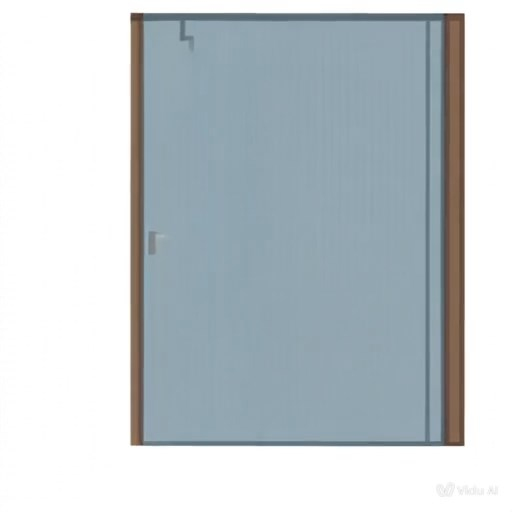
\includegraphics[width=0.4\linewidth]{figs/vidu/framePortaHorizontalMaior.jpg}
    \legend{\small Fonte: Elaborada pela autora, utilizando a ferramenta Vidu.}
\end{figure}

Para a porta marrom, apenas foi anexado ao quadro inicial o sprite dela aberta. Os resultados\footnote{\url{https://drive.google.com/drive/folders/1EOloiSlzuRKM0gus7U78opbw4Q6lfjr-?usp=sharing}} não foram satisfatórios. No primeiro vídeo, a porta abre pelo lado direito (oposto ao correto) como uma sanfona (Figura \ref{fig:viduPortaSanfona}), com o sprite da porta ao lado dele mesmo mais escuro, ambos inclinados formando uma ponta. Por causa disso, o prompt foi ajustado para especificar que a porta deveria abrir para o lado esquerdo. Mesmo assim, o resultado não foi preciso. A porta continuou abrindo do lado errado, além de desconectar-se da moldura no começo da animação (Figura \ref{fig:viduPortaDesconexao}). Uma melhora em relação à animação anterior foi que o frame final gerou a porta aberta quase sem nenhuma inconsistência (Figura \ref{fig:viduPortaAberta}). O processo completo para geração das animações das portas pode ser consultado nas Figuras \ref{fig:vidu14} e \ref{fig:vidu15} no Apêndice \ref{ap.telasIA}.

\begin{figure}[htbp]
    \centering
    \begin{minipage}{0.32\textwidth}
    \centering
    \caption{\small Quadro da porta parecendo uma sanfona}
    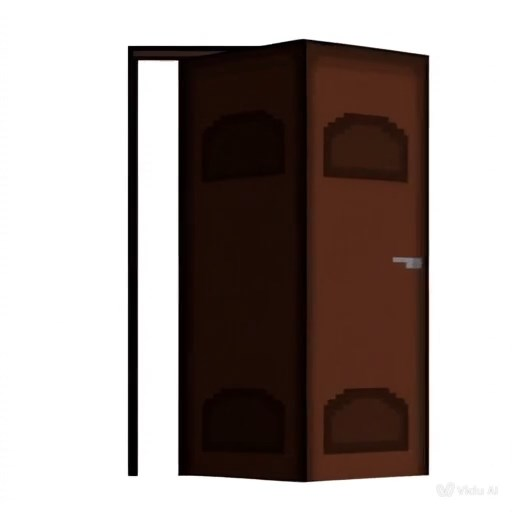
\includegraphics[width=1\linewidth]{figs/vidu/framePortaSanfona.jpg}
    \label{fig:viduPortaSanfona}
    \legend{\small Fonte: Elaborada pela autora, utilizando a ferramenta Vidu.}
    \end{minipage}\hfill
    \begin{minipage}{0.32\textwidth}
    \centering
    \caption{\small Quadro da porta desconectando da moldura}    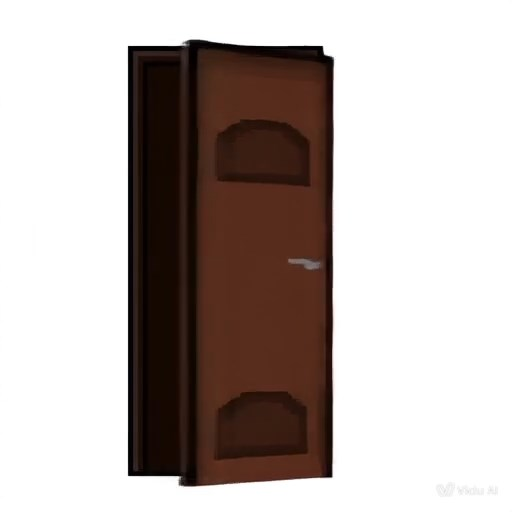
\includegraphics[width=1\linewidth]{figs/vidu/framePortaDesconexao.jpg}
    \label{fig:viduPortaDesconexao}
    \legend{\small Fonte: Elaborada pela autora, utilizando a ferramenta Vidu.}
    \end{minipage}\hfill
    \begin{minipage}{0.32\textwidth}
    \centering
    \caption{\small Quadro da porta aberta gerado no Vidu}    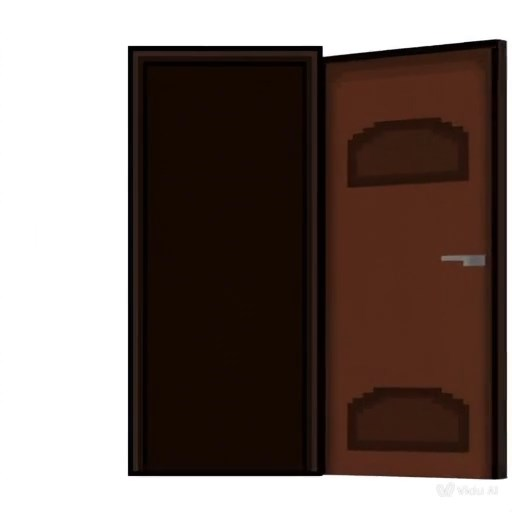
\includegraphics[width=1\linewidth]{figs/vidu/framePortaAberta.jpg}
    \label{fig:viduPortaAberta}
    \legend{\small Fonte: Elaborada pela autora, utilizando a ferramenta Vidu.}
    \end{minipage}\hfill
\end{figure}

No teste seguinte, o objetivo foi gerar uma animação para o pulo do personagem, visto que foi encontrada uma animação adequada para a porta marrom. O resultado\footnote{\url{https://drive.google.com/file/d/1QcPnZp21dFyTtQ_J57pV7zzT_W0MR8Js/view?usp=sharing}} foi extremamente insatisfatório, sem o movimento do pulo sequer ser gerado. No vídeo, o personagem dobra as pernas sem realmente se agachar e abre os braços, se inclinando para frente enquanto o fundo fica metade preto e os quadros ficam borrados (Figura \ref{fig:viduPuloInclina}).

\begin{figure}[htbp]
    \centering
    \caption{\small Quadro do personagem inclinando para frente na animação gerada no Vidu}
    \label{fig:viduPuloInclina}
    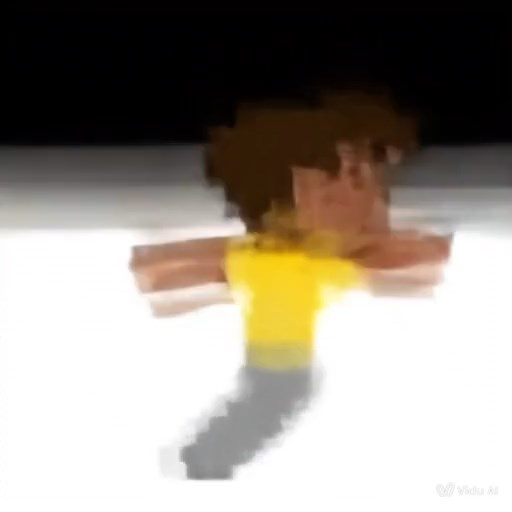
\includegraphics[width=0.4\linewidth]{figs/vidu/framePulo2.jpg}
    \legend{\small Fonte: Elaborada pela autora, utilizando a ferramenta Vidu.}
\end{figure}

A hipótese elaborada para a animação ter sido completamente imprecisa e com mudanças extras foi que, sem o frame final, a IA tem mais dificuldade em fazer movimentos onde a cena não acaba diferente do quadro inicial. O pulo não é um movimento linear: o personagem chega a um ponto mais alto e depois cai até a mesma altura em que se estava antes. Porém, a funcionalidade parece ter sido feita para mostrar uma progressão na transformação, chegar de um estado A para B sem nenhum terceiro ponto no caminho. Dessa forma, em busca de gerar uma mudança que gerasse uma progressão, foi modificado o fundo com o personagem apenas inclinando-se para frente em vez de fazer o movimento de ir para cima e depois para baixo.


Após algumas pesquisas mais aprofundadas na ferramenta, foi descoberto que os prompts para essa funcionalidade específica não funcionavam da mesma maneira que os do resto da ferramenta. É recomendado utilizar prompts curtos e visuais, mencionando o movimento da câmera e o estilo visual \cite{docs2_2025}. As sugestões foram feitas especificamente para o modelo Vidu Q1, porém, como citado anteriormente, o teste foi realizado no modelo Vidu 2.0.

Assim, durante o último teste, com o objetivo de gerar a animação da porta marrom em side view abrindo, é utilizado um prompt seguindo esse padrão. O resultado\footnote{\url{https://drive.google.com/file/d/1NfyI0P6tybE1VX_NeIegRJdKDVumBqmA/view?usp=sharing}} foi satisfatório, porém ele teria que passar por alguns ajustes antes de poder ser aplicado no jogo. A animação fez o movimento da porta abrindo, porém sem mover a maçaneta de lugar, como pode ser visto na Figura \ref{fig:viduPortaFinalAberta}.

\begin{figure}[htbp]
    \centering
    \caption{\small Porta em side view aberta na animação gerada no Vidu}
    \label{fig:viduPortaFinalAberta}
    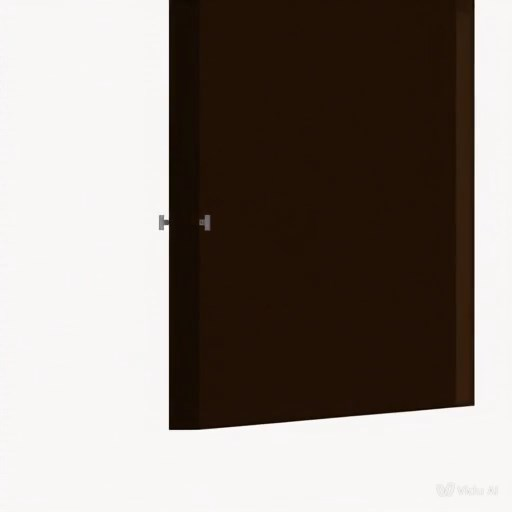
\includegraphics[width=0.4\linewidth]{figs/vidu/frameFinal.jpg}
    \legend{\small Fonte: Elaborada pela autora, utilizando a ferramenta Vidu.}
\end{figure}

Após o vídeo ter sido baixado, foi extraído seu sprite sheet pelo site ezgif (mencionado anteriormente) para ser possível fazer os ajustes com mais facilidade. Após isso, foi aberta a imagem no Pixilart (também mencionado anteriormente), transformando-a em uma verdadeira pixel art (Figura \ref{fig:viduPortaFinalSpriteSheetPixel}) onde seu fundo foi removido. Após isso, a animação estava pronta para ser exportada para a ferramenta Pixel Lab, onde foi realizado o pós-processamento (detalhado na Seção \ref{s.pixelLab}).

\begin{figure}[htbp]
    \centering
    \caption{\small Sprite sheet em pixel sem fundo da animação da porta em side view abrindo}
    \label{fig:viduPortaFinalSpriteSheetPixel}
    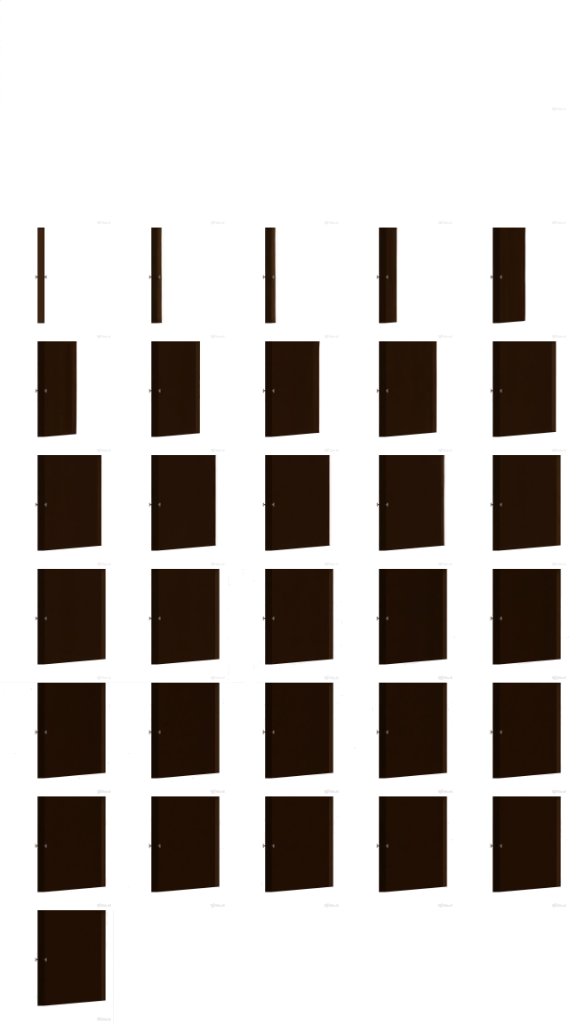
\includegraphics[width=0.4\linewidth]{figs/vidu/Pixilart/porta_sprite_sheet_pixel.png}
    \legend{\small Fonte: Elaborada pela autora, utilizando a ferramenta Pixilart.}
\end{figure}

Conclui-se que essa funcionalidade específica, ao trabalhar com frames definidos, suaviza a dificuldade da ferramenta em manter a consistência em 2D, observada na análise anterior. As falhas apresentadas foram relacionadas à imprecisão da interpretação do prompt e a uma aparente limitação com movimento de progressão não linear, como o pulo. A ferramenta demonstrou grande potencial e consistência para gerar um movimento fluído entre quadros-chave já desenhados, produzindo resultados que, embora precisem de ajustes finos, tornam o processo de animação mais eficiente.

